%
% fig/bisektion.tex -- Bisektion auf R
%
\begin{figure}
\centering
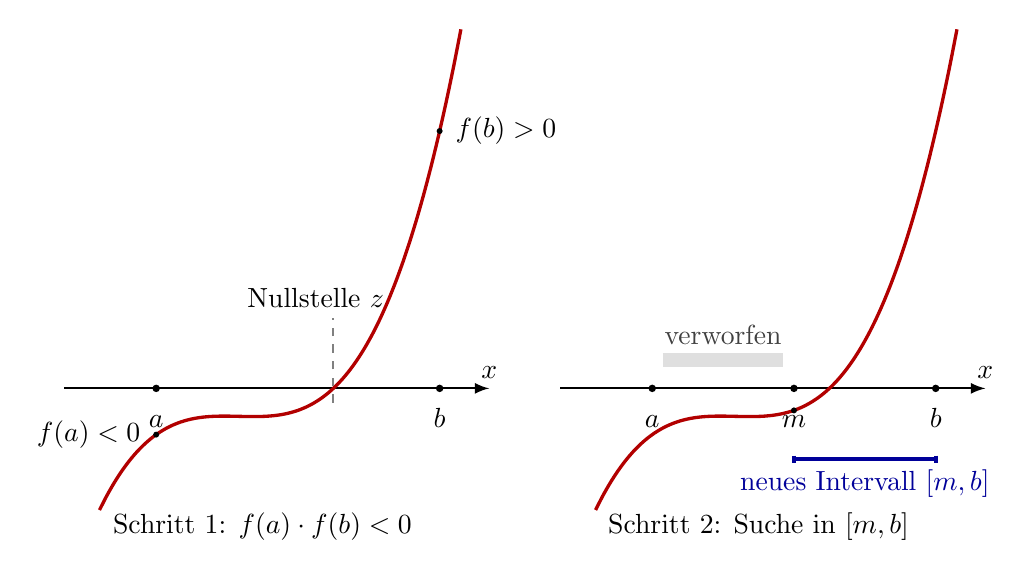
\begin{tikzpicture}[>=latex,thick,scale=0.9]
%
% Zwei Schritte der Bisektion nebeneinander
%
% --- Schritt 1: a, b mit Vorzeichenwechsel ---
\begin{scope}[xshift=0cm]
  % Achse
  \draw[->] (-0.3,0) -- (5.7,0) coordinate[label={above:$x$}];
  % Funktion: kubisch mit Nullstelle bei ca x = 3.5
  \draw[color=red!70!black,line width=1.2pt,smooth,samples=50,domain=0.2:5.3]
    plot (\x, {0.18*(\x-3.5)*((\x-1.5)*(\x-1.5)+1.2)});
  % Endpunkte a und b
  \fill (1,0) circle (1.5pt);
  \fill (5,0) circle (1.5pt);
  \node[below=3pt] at (1,0) {$a\mathstrut$};
  \node[below=3pt] at (5,0) {$b\mathstrut$};
  % Funktionswerte mit + und -
  \fill (1,{0.18*(1-3.5)*((1-1.5)*(1-1.5)+1.2)}) circle (1.2pt);
  \fill (5,{0.18*(5-3.5)*((5-1.5)*(5-1.5)+1.2)}) circle (1.2pt);
  \node[left=2pt] at (1,{0.18*(1-3.5)*((1-1.5)*(1-1.5)+1.2)}) {$f(a)<0$};
  \node[right=2pt] at (5,{0.18*(5-3.5)*((5-1.5)*(5-1.5)+1.2)}) {$f(b)>0$};
  % Nullstelle markieren
  \draw[dashed,gray] (3.5,-0.2) -- (3.5,1.0);
  \node[above] at (3.25,1.0) {Nullstelle $z$};
  \node at (2.5,-1.95) {Schritt 1: $f(a)\cdot f(b) < 0$};
\end{scope}
%
% --- Schritt 2: Halbiert, m und b ---
\begin{scope}[xshift=7cm]
  \draw[->] (-0.3,0) -- (5.7,0) coordinate[label={above:$x$}];
  \draw[color=red!70!black,line width=1.2pt,smooth,samples=50,domain=0.2:5.3]
    plot (\x, {0.18*(\x-3.5)*((\x-1.5)*(\x-1.5)+1.2)});
  % Mittelpunkt m=3, neue Endpunkte m und b=5
  \fill (1,0) circle (1.5pt);
  \fill (3,0) circle (1.5pt);
  \fill (5,0) circle (1.5pt);
  \node[below=3pt] at (1,0) {$a\mathstrut$};
  \node[below=3pt] at (3,0) {$m\mathstrut$};
  \node[below=3pt] at (5,0) {$b\mathstrut$};
  % Linke Hälfte (verworfen): grauer Querbalken oberhalb der Achse
  \draw[gray!50,line width=5pt,opacity=0.5] (1.15,0.4) -- (2.85,0.4);
  \node[gray!50!black] at (2,0.75) {verworfen};
  % Funktionswert bei m (Punkt ohne Label, Position spricht für sich)
  \fill (3,{0.18*(3-3.5)*((3-1.5)*(3-1.5)+1.2)}) circle (1.2pt);
  % Neuer Suchbereich
  \draw[blue!60!black,line width=1.5pt] (3,-1.0) -- (5,-1.0);
  \draw[blue!60!black,line width=1.5pt] (3,-0.95) -- (3,-1.05);
  \draw[blue!60!black,line width=1.5pt] (5,-0.95) -- (5,-1.05);
  \node[blue!60!black] at (4,-1.35) {neues Intervall $[m,b]$};
  \node at (2.5,-1.95) {Schritt 2: Suche in $[m,b]$};
\end{scope}
\end{tikzpicture}
\caption{Bisektion einer reellen stetigen Funktion: das Vorzeichen wechselt
zwischen $a$ und $b$, also liegt nach dem Zwischenwertsatz mindestens eine
Nullstelle dazwischen. Durch Halbieren und Auswählen der Hälfte mit
Vorzeichenwechsel verkleinert sich der Suchbereich pro Schritt um den Faktor zwei.
\label{weyl:fig:bisektion}}
\end{figure}
